% J. S. Morrison - J. R. Capablanca, New York, 1918, with Capablanca's notes.
% Build with: python3 ../../tools/chessbook.py game-13-morrison-capablanca.tex
\documentclass[10pt,twoside]{article}
\usepackage[paperwidth=487.56bp,paperheight=691.65bp,top=72pt,bottom=44pt,inner=50pt,outer=48pt,
            headheight=13pt,headsep=20pt,footskip=0pt]{geometry}
\usepackage[T1]{fontenc}
\usepackage[lining]{ebgaramond}
\usepackage{graphicx}
\usepackage{microtype}
\usepackage{tikz}
\usepackage{fancyhdr}
\usepackage[hidelinks,pdftitle={Morrison - Capablanca, New York, 1918},
            pdfauthor={J. R. Capablanca}]{hyperref}

\newcommand{\textsizebook}{\fontsize{10.5}{12.6}\selectfont}
\AtBeginDocument{\textsizebook}
\setlength{\columnsep}{11pt}
\setlength{\parindent}{9pt}
\setlength{\parskip}{0pt}
\setlength{\emergencystretch}{1.5em}
\raggedbottom

\newlength{\boardwidth}
\setlength{\boardwidth}{160pt}

% A main line move, as a bold heading above its note
\newcommand{\Move}[1]{\par\addvspace{8pt}\noindent\phantomsection{\bfseries #1}\par\nopagebreak}
% A diagram in the text
\newcommand{\ChessDiagram}[1]{\par\addvspace{7pt}{\centering #1\par}\addvspace{5pt}}

\pagestyle{fancy}
\fancyhf{}
\renewcommand{\headrulewidth}{0pt}
\fancyhead[LE,RO]{\thepage}
\fancyhead[CE]{Ruy Lopez}
\fancyhead[CO]{Morrison -- Capablanca}






\newcommand{\figK}{\raisebox{-0.14em}{
\includegraphics[height=1em]{diagrams/figK}}}
\newcommand{\figQ}{\raisebox{-0.14em}{
\includegraphics[height=1em]{diagrams/figQ}}}
\newcommand{\figR}{\raisebox{-0.14em}{
\includegraphics[height=1em]{diagrams/figR}}}
\newcommand{\figB}{\raisebox{-0.14em}{
\includegraphics[height=1em]{diagrams/figB}}}
\newcommand{\figN}{\raisebox{-0.14em}{
\includegraphics[height=1em]{diagrams/figN}}}
\begin{document}

\twocolumn[{%
\thispagestyle{empty}
\begin{tikzpicture}[remember picture,overlay]
  \node[circle,draw=black,line width=1.6pt,fill=black!20,minimum size=112pt] (seal)
       at ([xshift=75pt,yshift=-75pt]current page.north west) {};
  \draw[line width=0.9pt] ([shift={(-48pt,-30pt)}]seal.center) -- ([shift={(44pt,34pt)}]seal.center);
  \node[rotate=37] at ([shift={(-11pt,14pt)}]seal.center) {\fontsize{25}{25}\selectfont\bfseries Game};
  \node[rotate=37] at ([shift={(10pt,-16pt)}]seal.center) {\fontsize{38}{38}\selectfont\bfseries 13};
  \node[anchor=north east] at ([xshift=-14pt,yshift=-24pt]current page.north east)
       {\href{https://lichess.org/analysis/pgn/e4_e5_Nf3_Nc6_Bb5_d6_Nc3_Bd7}{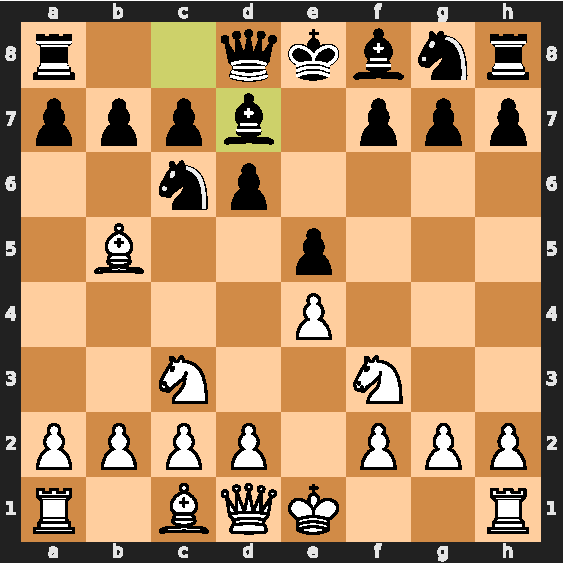
\includegraphics[width=108pt]{diagrams/board-aa1266f3532d}}};
\end{tikzpicture}

\vspace*{38pt}
\begin{center}
  \begin{minipage}{235pt}\centering
    {\fontsize{22}{25}\selectfont\bfseries Ruy Lopez\par}
    \vspace{4pt}\rule{\linewidth}{1pt}\\[-9.5pt]\rule{\linewidth}{0.4pt}
  \end{minipage}

  \vspace{14pt}
  {\fontsize{19}{22}\selectfont\bfseries Morrison -- Capablanca\par}
  \vspace{10pt}
  {\fontsize{15}{18}\selectfont\bfseries New York, 1918\par}
  \vspace{8pt}
  {\fontsize{11}{13}\selectfont White: J. S. Morrison \quad Black: J. R. Capablanca\par}
  \vspace{10pt}
  {\centering\fontsize{8.5}{10}\selectfont\itshape
   Notes by J. R. Capablanca, from \textup{Chess Fundamentals} (1921), which is in the public domain.\\
   Descriptive notation has been converted to algebraic. Page references are to the book.\\
   Click any move or diagram to open it on Lichess.\par}
\end{center}
\vspace{10pt}
}]
\textsizebook

\Move{\href{https://lichess.org/analysis/pgn/e4}{1.e4} \href{https://lichess.org/analysis/pgn/e4_e5}{e5} \href{https://lichess.org/analysis/pgn/e4_e5_Nf3}{2.\figN f3} \href{https://lichess.org/analysis/pgn/e4_e5_Nf3_Nc6}{\figN c6} \href{https://lichess.org/analysis/pgn/e4_e5_Nf3_Nc6_Bb5}{3.\figB b5} \href{https://lichess.org/analysis/pgn/e4_e5_Nf3_Nc6_Bb5_d6}{d6} \href{https://lichess.org/analysis/pgn/e4_e5_Nf3_Nc6_Bb5_d6_Nc3}{4.\figN c3} \href{https://lichess.org/analysis/pgn/e4_e5_Nf3_Nc6_Bb5_d6_Nc3_Bd7}{\figB d7} \href{https://lichess.org/analysis/pgn/e4_e5_Nf3_Nc6_Bb5_d6_Nc3_Bd7_d4}{5.d4} \href{https://lichess.org/analysis/pgn/e4_e5_Nf3_Nc6_Bb5_d6_Nc3_Bd7_d4_exd4}{exd4} \href{https://lichess.org/analysis/pgn/e4_e5_Nf3_Nc6_Bb5_d6_Nc3_Bd7_d4_exd4_Nxd4}{6.\figN xd4} \href{https://lichess.org/analysis/pgn/e4_e5_Nf3_Nc6_Bb5_d6_Nc3_Bd7_d4_exd4_Nxd4_g6}{g6}}

In this form of defence of the Ruy Lopez the development of the King's Bishop via g7 is, I think, of great importance. The Bishop at g7 exerts great pressure along the long diagonal. At the same time the position of the Bishop and Pawns in front of the King, once it is Castled, is one of great defensive strength. Therefore, in this form of development, the Bishop, we might say, exerts its maximum strength (Compare this note with the one in the Capablanca-Burn game at San Sebastian, page 197.)

\Move{\href{https://lichess.org/analysis/pgn/e4_e5_Nf3_Nc6_Bb5_d6_Nc3_Bd7_d4_exd4_Nxd4_g6_Nf3}{7.\figN f3} \href{https://lichess.org/analysis/pgn/e4_e5_Nf3_Nc6_Bb5_d6_Nc3_Bd7_d4_exd4_Nxd4_g6_Nf3_Bg7}{\figB g7} \href{https://lichess.org/analysis/pgn/e4_e5_Nf3_Nc6_Bb5_d6_Nc3_Bd7_d4_exd4_Nxd4_g6_Nf3_Bg7_Bg5}{8.\figB g5} \href{https://lichess.org/analysis/pgn/e4_e5_Nf3_Nc6_Bb5_d6_Nc3_Bd7_d4_exd4_Nxd4_g6_Nf3_Bg7_Bg5_Nf6}{\figN f6}}

Of course not \href{https://lichess.org/analysis/pgn/e4_e5_Nf3_Nc6_Bb5_d6_Nc3_Bd7_d4_exd4_Nxd4_g6_Nf3_Bg7_Bg5_Nge7}{8...\figN ge7}; because of \href{https://lichess.org/analysis/pgn/e4_e5_Nf3_Nc6_Bb5_d6_Nc3_Bd7_d4_exd4_Nxd4_g6_Nf3_Bg7_Bg5_Nge7_Nd5}{9.\figN d5}. The alternative would have been \href{https://lichess.org/analysis/pgn/e4_e5_Nf3_Nc6_Bb5_d6_Nc3_Bd7_d4_exd4_Nxd4_g6_Nf3_Bg7_Bg5_f6}{8...f6}; to be followed by \figN ge7; but in this position it is preferable to have the Knight at f6.

\Move{\href{https://lichess.org/analysis/pgn/e4_e5_Nf3_Nc6_Bb5_d6_Nc3_Bd7_d4_exd4_Nxd4_g6_Nf3_Bg7_Bg5_Nf6_Qd2}{9.\figQ d2} \href{https://lichess.org/analysis/pgn/e4_e5_Nf3_Nc6_Bb5_d6_Nc3_Bd7_d4_exd4_Nxd4_g6_Nf3_Bg7_Bg5_Nf6_Qd2_h6}{h6} \href{https://lichess.org/analysis/pgn/e4_e5_Nf3_Nc6_Bb5_d6_Nc3_Bd7_d4_exd4_Nxd4_g6_Nf3_Bg7_Bg5_Nf6_Qd2_h6_Bh4}{10.\figB h4}}

An error of judgment. White wants to keep the Knight pinned, but it was more important to prevent Black from Castling immediately. \href{https://lichess.org/analysis/pgn/e4_e5_Nf3_Nc6_Bb5_d6_Nc3_Bd7_d4_exd4_Nxd4_g6_Nf3_Bg7_Bg5_Nf6_Qd2_h6_Bf4}{10.\figB f4} would have done this.

\Move{\href{https://lichess.org/analysis/pgn/e4_e5_Nf3_Nc6_Bb5_d6_Nc3_Bd7_d4_exd4_Nxd4_g6_Nf3_Bg7_Bg5_Nf6_Qd2_h6_Bh4_O-O}{10...0--0} \href{https://lichess.org/analysis/pgn/e4_e5_Nf3_Nc6_Bb5_d6_Nc3_Bd7_d4_exd4_Nxd4_g6_Nf3_Bg7_Bg5_Nf6_Qd2_h6_Bh4_O-O_O-O-O}{11.0--0--0}}

Bold play, but again faulty judgment, unless he intended to play to win or lose, throwing safety to the winds. The Black Bishop at g7 becomes a very powerful attacking piece. The strategical disposition of the Black pieces is now far superior to White's, therefore it will be Black who will take the offensive.

\Move{\href{https://lichess.org/analysis/pgn/e4_e5_Nf3_Nc6_Bb5_d6_Nc3_Bd7_d4_exd4_Nxd4_g6_Nf3_Bg7_Bg5_Nf6_Qd2_h6_Bh4_O-O_O-O-O_Re8}{11...\figR e8} \href{https://lichess.org/analysis/pgn/e4_e5_Nf3_Nc6_Bb5_d6_Nc3_Bd7_d4_exd4_Nxd4_g6_Nf3_Bg7_Bg5_Nf6_Qd2_h6_Bh4_O-O_O-O-O_Re8_Rhe1}{12.\figR he1}}

\ChessDiagram{\href{https://lichess.org/analysis/pgn/e4_e5_Nf3_Nc6_Bb5_d6_Nc3_Bd7_d4_exd4_Nxd4_g6_Nf3_Bg7_Bg5_Nf6_Qd2_h6_Bh4_O-O_O-O-O_Re8_Rhe1}{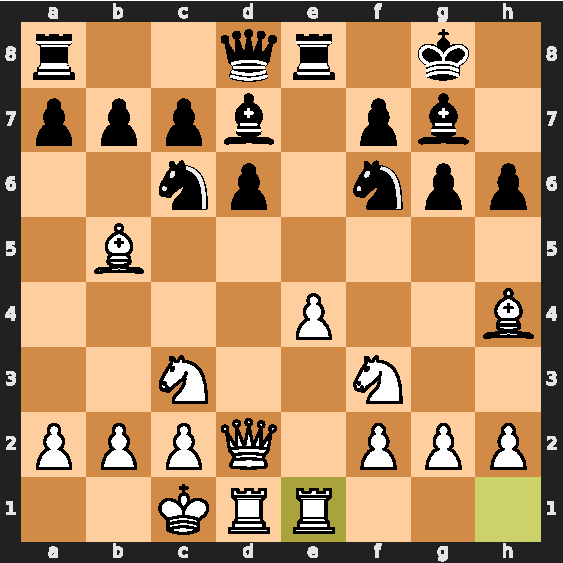
\includegraphics[width=\boardwidth]{diagrams/board-7de842e8dce2}}}

White wanted to keep his Queen's Rook on the open file, and consequently brings over his other Rook to the centre to defend his e-pawn, which Black threatened to win by ...g5, followed by \figN xe4.

\Move{\href{https://lichess.org/analysis/pgn/e4_e5_Nf3_Nc6_Bb5_d6_Nc3_Bd7_d4_exd4_Nxd4_g6_Nf3_Bg7_Bg5_Nf6_Qd2_h6_Bh4_O-O_O-O-O_Re8_Rhe1_g5}{12...g5!}}

Now that the King's Rook is in the centre, Black can safely advance, since, in order to attack on the King's side, White would have to shift his Rooks, which he cannot do so long as Black keeps up the pressure in the centre.

\Move{\href{https://lichess.org/analysis/pgn/e4_e5_Nf3_Nc6_Bb5_d6_Nc3_Bd7_d4_exd4_Nxd4_g6_Nf3_Bg7_Bg5_Nf6_Qd2_h6_Bh4_O-O_O-O-O_Re8_Rhe1_g5_Bg3}{13.\figB g3} \href{https://lichess.org/analysis/pgn/e4_e5_Nf3_Nc6_Bb5_d6_Nc3_Bd7_d4_exd4_Nxd4_g6_Nf3_Bg7_Bg5_Nf6_Qd2_h6_Bh4_O-O_O-O-O_Re8_Rhe1_g5_Bg3_Nh5}{\figN h5}}

Uncovering the Bishop, which now acts along the long diagonal, and at the same time preventing e5, which would be answered by \figN xg3; Pawn takes Knight, \figN xe5; etc., winning a Pawn.

\Move{\href{https://lichess.org/analysis/pgn/e4_e5_Nf3_Nc6_Bb5_d6_Nc3_Bd7_d4_exd4_Nxd4_g6_Nf3_Bg7_Bg5_Nf6_Qd2_h6_Bh4_O-O_O-O-O_Re8_Rhe1_g5_Bg3_Nh5_Nd5}{14.\figN d5} \href{https://lichess.org/analysis/pgn/e4_e5_Nf3_Nc6_Bb5_d6_Nc3_Bd7_d4_exd4_Nxd4_g6_Nf3_Bg7_Bg5_Nf6_Qd2_h6_Bh4_O-O_O-O-O_Re8_Rhe1_g5_Bg3_Nh5_Nd5_a6}{a6}}

Black drives the Bishop away so as to \emph{unpin} his pieces and be able to manoeuvre freely.

\Move{\href{https://lichess.org/analysis/pgn/e4_e5_Nf3_Nc6_Bb5_d6_Nc3_Bd7_d4_exd4_Nxd4_g6_Nf3_Bg7_Bg5_Nf6_Qd2_h6_Bh4_O-O_O-O-O_Re8_Rhe1_g5_Bg3_Nh5_Nd5_a6_Bd3}{15.\figB d3} \href{https://lichess.org/analysis/pgn/e4_e5_Nf3_Nc6_Bb5_d6_Nc3_Bd7_d4_exd4_Nxd4_g6_Nf3_Bg7_Bg5_Nf6_Qd2_h6_Bh4_O-O_O-O-O_Re8_Rhe1_g5_Bg3_Nh5_Nd5_a6_Bd3_Be6}{\figB e6}}

Preparing the onslaught. Black's pieces begin to bear against the King's position.

\Move{\href{https://lichess.org/analysis/pgn/e4_e5_Nf3_Nc6_Bb5_d6_Nc3_Bd7_d4_exd4_Nxd4_g6_Nf3_Bg7_Bg5_Nf6_Qd2_h6_Bh4_O-O_O-O-O_Re8_Rhe1_g5_Bg3_Nh5_Nd5_a6_Bd3_Be6_c3}{16.c3}}

\ChessDiagram{\href{https://lichess.org/analysis/pgn/e4_e5_Nf3_Nc6_Bb5_d6_Nc3_Bd7_d4_exd4_Nxd4_g6_Nf3_Bg7_Bg5_Nf6_Qd2_h6_Bh4_O-O_O-O-O_Re8_Rhe1_g5_Bg3_Nh5_Nd5_a6_Bd3_Be6_c3}{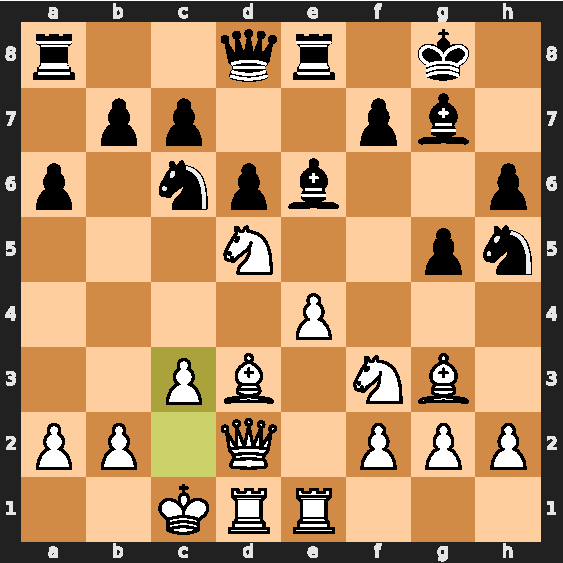
\includegraphics[width=\boardwidth]{diagrams/board-745f3934986f}}}

With the last move White not only blocks the action of Black's King's Bishop, but he also aims at placing his Bishop at b1 and his Queen at c2, and then advancing his e-pawn, to check at h7.

\Move{\href{https://lichess.org/analysis/pgn/e4_e5_Nf3_Nc6_Bb5_d6_Nc3_Bd7_d4_exd4_Nxd4_g6_Nf3_Bg7_Bg5_Nf6_Qd2_h6_Bh4_O-O_O-O-O_Re8_Rhe1_g5_Bg3_Nh5_Nd5_a6_Bd3_Be6_c3_f5}{16...f5!}}

Initiating an attack to which there is no reply, and which has for its ultimate object either the winning of the White Queen's Bishop or cutting it off from the game. (Compare this game with the Winter-Capablanca game at Hastings.)

\Move{\href{https://lichess.org/analysis/pgn/e4_e5_Nf3_Nc6_Bb5_d6_Nc3_Bd7_d4_exd4_Nxd4_g6_Nf3_Bg7_Bg5_Nf6_Qd2_h6_Bh4_O-O_O-O-O_Re8_Rhe1_g5_Bg3_Nh5_Nd5_a6_Bd3_Be6_c3_f5_h4}{17.h4} \href{https://lichess.org/analysis/pgn/e4_e5_Nf3_Nc6_Bb5_d6_Nc3_Bd7_d4_exd4_Nxd4_g6_Nf3_Bg7_Bg5_Nf6_Qd2_h6_Bh4_O-O_O-O-O_Re8_Rhe1_g5_Bg3_Nh5_Nd5_a6_Bd3_Be6_c3_f5_h4_f4}{f4}}

The Bishop is now out of action. White naturally counter attacks violently against the seemingly exposed position of the Black King, and, with very good judgment, even offers the Bishop.

\ChessDiagram{\href{https://lichess.org/analysis/pgn/e4_e5_Nf3_Nc6_Bb5_d6_Nc3_Bd7_d4_exd4_Nxd4_g6_Nf3_Bg7_Bg5_Nf6_Qd2_h6_Bh4_O-O_O-O-O_Re8_Rhe1_g5_Bg3_Nh5_Nd5_a6_Bd3_Be6_c3_f5_h4_f4}{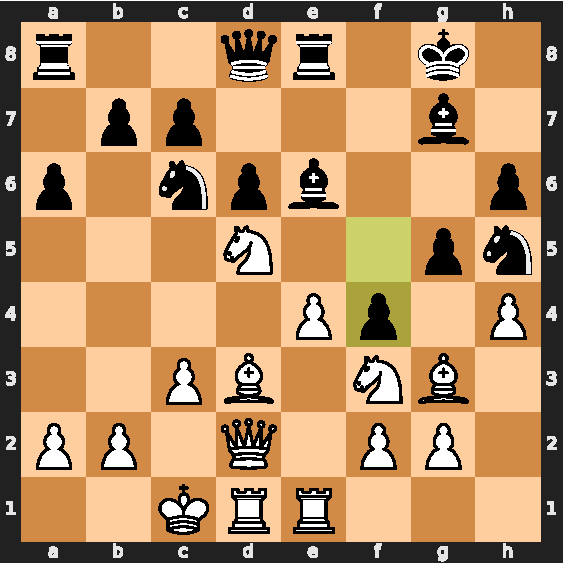
\includegraphics[width=\boardwidth]{diagrams/board-69199059ef1e}}}

\Move{\href{https://lichess.org/analysis/pgn/e4_e5_Nf3_Nc6_Bb5_d6_Nc3_Bd7_d4_exd4_Nxd4_g6_Nf3_Bg7_Bg5_Nf6_Qd2_h6_Bh4_O-O_O-O-O_Re8_Rhe1_g5_Bg3_Nh5_Nd5_a6_Bd3_Be6_c3_f5_h4_f4_hxg5}{18.hxg5!} \href{https://lichess.org/analysis/pgn/e4_e5_Nf3_Nc6_Bb5_d6_Nc3_Bd7_d4_exd4_Nxd4_g6_Nf3_Bg7_Bg5_Nf6_Qd2_h6_Bh4_O-O_O-O-O_Re8_Rhe1_g5_Bg3_Nh5_Nd5_a6_Bd3_Be6_c3_f5_h4_f4_hxg5_hxg5}{hxg5!}}

Taking the Bishop would be dangerous, if not actually bad, while the text move accomplishes Black's object, which is to put the Bishop out of action.

\Move{\href{https://lichess.org/analysis/pgn/e4_e5_Nf3_Nc6_Bb5_d6_Nc3_Bd7_d4_exd4_Nxd4_g6_Nf3_Bg7_Bg5_Nf6_Qd2_h6_Bh4_O-O_O-O-O_Re8_Rhe1_g5_Bg3_Nh5_Nd5_a6_Bd3_Be6_c3_f5_h4_f4_hxg5_hxg5_Rh1}{19.\figR h1} \href{https://lichess.org/analysis/pgn/e4_e5_Nf3_Nc6_Bb5_d6_Nc3_Bd7_d4_exd4_Nxd4_g6_Nf3_Bg7_Bg5_Nf6_Qd2_h6_Bh4_O-O_O-O-O_Re8_Rhe1_g5_Bg3_Nh5_Nd5_a6_Bd3_Be6_c3_f5_h4_f4_hxg5_hxg5_Rh1_Bf7}{\figB f7} \href{https://lichess.org/analysis/pgn/e4_e5_Nf3_Nc6_Bb5_d6_Nc3_Bd7_d4_exd4_Nxd4_g6_Nf3_Bg7_Bg5_Nf6_Qd2_h6_Bh4_O-O_O-O-O_Re8_Rhe1_g5_Bg3_Nh5_Nd5_a6_Bd3_Be6_c3_f5_h4_f4_hxg5_hxg5_Rh1_Bf7_Kb1}{20.\figK b1}}

This move unquestionably loses time. Since he would have to retire his Bishop to h2 sooner or later, he might have done it immediately. It is doubtful, however, if at this stage of the game it would be possible for White to save the game.

\Move{\href{https://lichess.org/analysis/pgn/e4_e5_Nf3_Nc6_Bb5_d6_Nc3_Bd7_d4_exd4_Nxd4_g6_Nf3_Bg7_Bg5_Nf6_Qd2_h6_Bh4_O-O_O-O-O_Re8_Rhe1_g5_Bg3_Nh5_Nd5_a6_Bd3_Be6_c3_f5_h4_f4_hxg5_hxg5_Rh1_Bf7_Kb1_Ne5}{20...\figN e5} \href{https://lichess.org/analysis/pgn/e4_e5_Nf3_Nc6_Bb5_d6_Nc3_Bd7_d4_exd4_Nxd4_g6_Nf3_Bg7_Bg5_Nf6_Qd2_h6_Bh4_O-O_O-O-O_Re8_Rhe1_g5_Bg3_Nh5_Nd5_a6_Bd3_Be6_c3_f5_h4_f4_hxg5_hxg5_Rh1_Bf7_Kb1_Ne5_Nxe5}{21.\figN xe5} \href{https://lichess.org/analysis/pgn/e4_e5_Nf3_Nc6_Bb5_d6_Nc3_Bd7_d4_exd4_Nxd4_g6_Nf3_Bg7_Bg5_Nf6_Qd2_h6_Bh4_O-O_O-O-O_Re8_Rhe1_g5_Bg3_Nh5_Nd5_a6_Bd3_Be6_c3_f5_h4_f4_hxg5_hxg5_Rh1_Bf7_Kb1_Ne5_Nxe5_Rxe5}{\figR xe5}}

It was difficult to decide which way to retake. I took with the Rook in order to have it prepared for a possible attack against the King.

\Move{\href{https://lichess.org/analysis/pgn/e4_e5_Nf3_Nc6_Bb5_d6_Nc3_Bd7_d4_exd4_Nxd4_g6_Nf3_Bg7_Bg5_Nf6_Qd2_h6_Bh4_O-O_O-O-O_Re8_Rhe1_g5_Bg3_Nh5_Nd5_a6_Bd3_Be6_c3_f5_h4_f4_hxg5_hxg5_Rh1_Bf7_Kb1_Ne5_Nxe5_Rxe5_Bh2}{22.\figB h2} \href{https://lichess.org/analysis/pgn/e4_e5_Nf3_Nc6_Bb5_d6_Nc3_Bd7_d4_exd4_Nxd4_g6_Nf3_Bg7_Bg5_Nf6_Qd2_h6_Bh4_O-O_O-O-O_Re8_Rhe1_g5_Bg3_Nh5_Nd5_a6_Bd3_Be6_c3_f5_h4_f4_hxg5_hxg5_Rh1_Bf7_Kb1_Ne5_Nxe5_Rxe5_Bh2_Nf6}{\figN f6}}

Now that the White Bishop has been driven back, Black wants to get rid of White's strongly posted Knight at d5, which blocks the attack of the Bishop at f7. It may be said that the Knight at d5 is the key to White's defence.

\ChessDiagram{\href{https://lichess.org/analysis/pgn/e4_e5_Nf3_Nc6_Bb5_d6_Nc3_Bd7_d4_exd4_Nxd4_g6_Nf3_Bg7_Bg5_Nf6_Qd2_h6_Bh4_O-O_O-O-O_Re8_Rhe1_g5_Bg3_Nh5_Nd5_a6_Bd3_Be6_c3_f5_h4_f4_hxg5_hxg5_Rh1_Bf7_Kb1_Ne5_Nxe5_Rxe5_Bh2_Nf6}{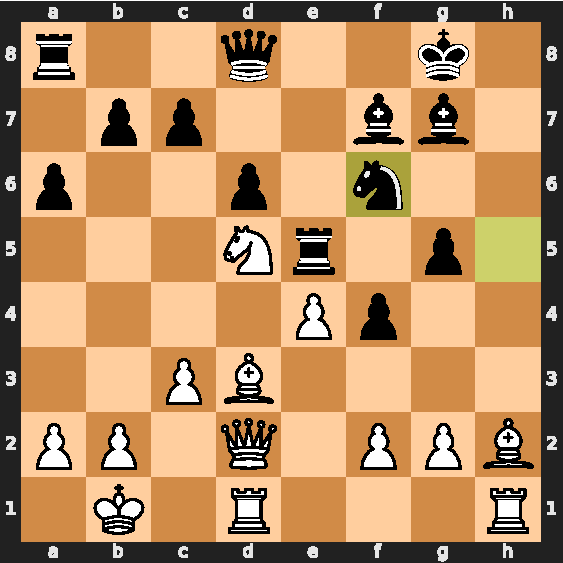
\includegraphics[width=\boardwidth]{diagrams/board-26ba767197b2}}}

\Move{\href{https://lichess.org/analysis/pgn/e4_e5_Nf3_Nc6_Bb5_d6_Nc3_Bd7_d4_exd4_Nxd4_g6_Nf3_Bg7_Bg5_Nf6_Qd2_h6_Bh4_O-O_O-O-O_Re8_Rhe1_g5_Bg3_Nh5_Nd5_a6_Bd3_Be6_c3_f5_h4_f4_hxg5_hxg5_Rh1_Bf7_Kb1_Ne5_Nxe5_Rxe5_Bh2_Nf6_g3}{23.g3}}

White strives not only to have play for his Bishop, but also he wants to break up Black's Pawns in order to counter-attack. The alternative would have been \href{https://lichess.org/analysis/pgn/e4_e5_Nf3_Nc6_Bb5_d6_Nc3_Bd7_d4_exd4_Nxd4_g6_Nf3_Bg7_Bg5_Nf6_Qd2_h6_Bh4_O-O_O-O-O_Re8_Rhe1_g5_Bg3_Nh5_Nd5_a6_Bd3_Be6_c3_f5_h4_f4_hxg5_hxg5_Rh1_Bf7_Kb1_Ne5_Nxe5_Rxe5_Bh2_Nf6_Nxf6}{23.\figN xf6+} \href{https://lichess.org/analysis/pgn/e4_e5_Nf3_Nc6_Bb5_d6_Nc3_Bd7_d4_exd4_Nxd4_g6_Nf3_Bg7_Bg5_Nf6_Qd2_h6_Bh4_O-O_O-O-O_Re8_Rhe1_g5_Bg3_Nh5_Nd5_a6_Bd3_Be6_c3_f5_h4_f4_hxg5_hxg5_Rh1_Bf7_Kb1_Ne5_Nxe5_Rxe5_Bh2_Nf6_Nxf6_Qxf6}{\figQ xf6}; and Black would be threatening \figR h5, and also \figQ e6. The student should notice that Black's drawback in all this is the fact that he is playing minus the services of his Queen's Rook. It is this fact that makes it possible for White to hold out longer.

\Move{\href{https://lichess.org/analysis/pgn/e4_e5_Nf3_Nc6_Bb5_d6_Nc3_Bd7_d4_exd4_Nxd4_g6_Nf3_Bg7_Bg5_Nf6_Qd2_h6_Bh4_O-O_O-O-O_Re8_Rhe1_g5_Bg3_Nh5_Nd5_a6_Bd3_Be6_c3_f5_h4_f4_hxg5_hxg5_Rh1_Bf7_Kb1_Ne5_Nxe5_Rxe5_Bh2_Nf6_g3_Nxe4}{23...\figN xe4} \href{https://lichess.org/analysis/pgn/e4_e5_Nf3_Nc6_Bb5_d6_Nc3_Bd7_d4_exd4_Nxd4_g6_Nf3_Bg7_Bg5_Nf6_Qd2_h6_Bh4_O-O_O-O-O_Re8_Rhe1_g5_Bg3_Nh5_Nd5_a6_Bd3_Be6_c3_f5_h4_f4_hxg5_hxg5_Rh1_Bf7_Kb1_Ne5_Nxe5_Rxe5_Bh2_Nf6_g3_Nxe4_Bxe4}{24.\figB xe4} \href{https://lichess.org/analysis/pgn/e4_e5_Nf3_Nc6_Bb5_d6_Nc3_Bd7_d4_exd4_Nxd4_g6_Nf3_Bg7_Bg5_Nf6_Qd2_h6_Bh4_O-O_O-O-O_Re8_Rhe1_g5_Bg3_Nh5_Nd5_a6_Bd3_Be6_c3_f5_h4_f4_hxg5_hxg5_Rh1_Bf7_Kb1_Ne5_Nxe5_Rxe5_Bh2_Nf6_g3_Nxe4_Bxe4_Rxe4}{\figR xe4} \href{https://lichess.org/analysis/pgn/e4_e5_Nf3_Nc6_Bb5_d6_Nc3_Bd7_d4_exd4_Nxd4_g6_Nf3_Bg7_Bg5_Nf6_Qd2_h6_Bh4_O-O_O-O-O_Re8_Rhe1_g5_Bg3_Nh5_Nd5_a6_Bd3_Be6_c3_f5_h4_f4_hxg5_hxg5_Rh1_Bf7_Kb1_Ne5_Nxe5_Rxe5_Bh2_Nf6_g3_Nxe4_Bxe4_Rxe4_gxf4}{25.gxf4} \href{https://lichess.org/analysis/pgn/e4_e5_Nf3_Nc6_Bb5_d6_Nc3_Bd7_d4_exd4_Nxd4_g6_Nf3_Bg7_Bg5_Nf6_Qd2_h6_Bh4_O-O_O-O-O_Re8_Rhe1_g5_Bg3_Nh5_Nd5_a6_Bd3_Be6_c3_f5_h4_f4_hxg5_hxg5_Rh1_Bf7_Kb1_Ne5_Nxe5_Rxe5_Bh2_Nf6_g3_Nxe4_Bxe4_Rxe4_gxf4_c6}{c6}}

\ChessDiagram{\href{https://lichess.org/analysis/pgn/e4_e5_Nf3_Nc6_Bb5_d6_Nc3_Bd7_d4_exd4_Nxd4_g6_Nf3_Bg7_Bg5_Nf6_Qd2_h6_Bh4_O-O_O-O-O_Re8_Rhe1_g5_Bg3_Nh5_Nd5_a6_Bd3_Be6_c3_f5_h4_f4_hxg5_hxg5_Rh1_Bf7_Kb1_Ne5_Nxe5_Rxe5_Bh2_Nf6_g3_Nxe4_Bxe4_Rxe4_gxf4_c6}{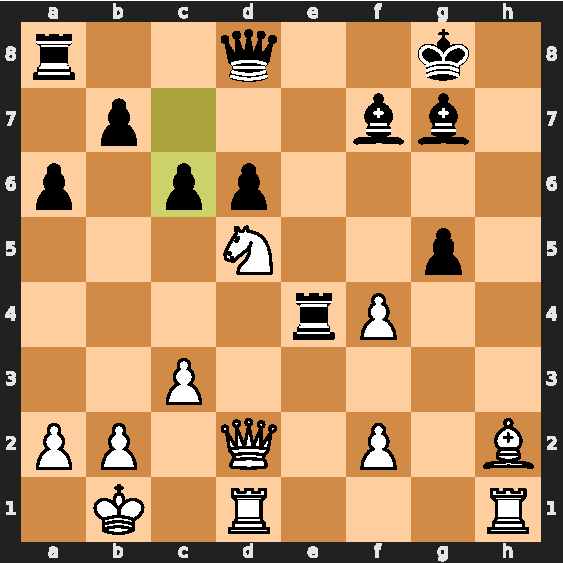
\includegraphics[width=\boardwidth]{diagrams/board-2e77ff5164b9}}}

\Move{\href{https://lichess.org/analysis/pgn/e4_e5_Nf3_Nc6_Bb5_d6_Nc3_Bd7_d4_exd4_Nxd4_g6_Nf3_Bg7_Bg5_Nf6_Qd2_h6_Bh4_O-O_O-O-O_Re8_Rhe1_g5_Bg3_Nh5_Nd5_a6_Bd3_Be6_c3_f5_h4_f4_hxg5_hxg5_Rh1_Bf7_Kb1_Ne5_Nxe5_Rxe5_Bh2_Nf6_g3_Nxe4_Bxe4_Rxe4_gxf4_c6_Ne3}{26.\figN e3}}

\href{https://lichess.org/analysis/pgn/e4_e5_Nf3_Nc6_Bb5_d6_Nc3_Bd7_d4_exd4_Nxd4_g6_Nf3_Bg7_Bg5_Nf6_Qd2_h6_Bh4_O-O_O-O-O_Re8_Rhe1_g5_Bg3_Nh5_Nd5_a6_Bd3_Be6_c3_f5_h4_f4_hxg5_hxg5_Rh1_Bf7_Kb1_Ne5_Nxe5_Rxe5_Bh2_Nf6_g3_Nxe4_Bxe4_Rxe4_gxf4_c6_Nb4}{26.\figN b4} was the alternative, but in any event White could not resist the attack. I leave it to the reader to work this out for himself, as the variations are so numerous that they would take up too much space.

\Move{\href{https://lichess.org/analysis/pgn/e4_e5_Nf3_Nc6_Bb5_d6_Nc3_Bd7_d4_exd4_Nxd4_g6_Nf3_Bg7_Bg5_Nf6_Qd2_h6_Bh4_O-O_O-O-O_Re8_Rhe1_g5_Bg3_Nh5_Nd5_a6_Bd3_Be6_c3_f5_h4_f4_hxg5_hxg5_Rh1_Bf7_Kb1_Ne5_Nxe5_Rxe5_Bh2_Nf6_g3_Nxe4_Bxe4_Rxe4_gxf4_c6_Ne3_Qa5}{26...\figQ a5} \href{https://lichess.org/analysis/pgn/e4_e5_Nf3_Nc6_Bb5_d6_Nc3_Bd7_d4_exd4_Nxd4_g6_Nf3_Bg7_Bg5_Nf6_Qd2_h6_Bh4_O-O_O-O-O_Re8_Rhe1_g5_Bg3_Nh5_Nd5_a6_Bd3_Be6_c3_f5_h4_f4_hxg5_hxg5_Rh1_Bf7_Kb1_Ne5_Nxe5_Rxe5_Bh2_Nf6_g3_Nxe4_Bxe4_Rxe4_gxf4_c6_Ne3_Qa5_c4}{27.c4} \href{https://lichess.org/analysis/pgn/e4_e5_Nf3_Nc6_Bb5_d6_Nc3_Bd7_d4_exd4_Nxd4_g6_Nf3_Bg7_Bg5_Nf6_Qd2_h6_Bh4_O-O_O-O-O_Re8_Rhe1_g5_Bg3_Nh5_Nd5_a6_Bd3_Be6_c3_f5_h4_f4_hxg5_hxg5_Rh1_Bf7_Kb1_Ne5_Nxe5_Rxe5_Bh2_Nf6_g3_Nxe4_Bxe4_Rxe4_gxf4_c6_Ne3_Qa5_c4_Qxd2}{\figQ xd2} \href{https://lichess.org/analysis/pgn/e4_e5_Nf3_Nc6_Bb5_d6_Nc3_Bd7_d4_exd4_Nxd4_g6_Nf3_Bg7_Bg5_Nf6_Qd2_h6_Bh4_O-O_O-O-O_Re8_Rhe1_g5_Bg3_Nh5_Nd5_a6_Bd3_Be6_c3_f5_h4_f4_hxg5_hxg5_Rh1_Bf7_Kb1_Ne5_Nxe5_Rxe5_Bh2_Nf6_g3_Nxe4_Bxe4_Rxe4_gxf4_c6_Ne3_Qa5_c4_Qxd2_Rxd2}{28.\figR xd2} \href{https://lichess.org/analysis/pgn/e4_e5_Nf3_Nc6_Bb5_d6_Nc3_Bd7_d4_exd4_Nxd4_g6_Nf3_Bg7_Bg5_Nf6_Qd2_h6_Bh4_O-O_O-O-O_Re8_Rhe1_g5_Bg3_Nh5_Nd5_a6_Bd3_Be6_c3_f5_h4_f4_hxg5_hxg5_Rh1_Bf7_Kb1_Ne5_Nxe5_Rxe5_Bh2_Nf6_g3_Nxe4_Bxe4_Rxe4_gxf4_c6_Ne3_Qa5_c4_Qxd2_Rxd2_gxf4}{gxf4} \href{https://lichess.org/analysis/pgn/e4_e5_Nf3_Nc6_Bb5_d6_Nc3_Bd7_d4_exd4_Nxd4_g6_Nf3_Bg7_Bg5_Nf6_Qd2_h6_Bh4_O-O_O-O-O_Re8_Rhe1_g5_Bg3_Nh5_Nd5_a6_Bd3_Be6_c3_f5_h4_f4_hxg5_hxg5_Rh1_Bf7_Kb1_Ne5_Nxe5_Rxe5_Bh2_Nf6_g3_Nxe4_Bxe4_Rxe4_gxf4_c6_Ne3_Qa5_c4_Qxd2_Rxd2_gxf4_Ng4}{29.\figN g4} \href{https://lichess.org/analysis/pgn/e4_e5_Nf3_Nc6_Bb5_d6_Nc3_Bd7_d4_exd4_Nxd4_g6_Nf3_Bg7_Bg5_Nf6_Qd2_h6_Bh4_O-O_O-O-O_Re8_Rhe1_g5_Bg3_Nh5_Nd5_a6_Bd3_Be6_c3_f5_h4_f4_hxg5_hxg5_Rh1_Bf7_Kb1_Ne5_Nxe5_Rxe5_Bh2_Nf6_g3_Nxe4_Bxe4_Rxe4_gxf4_c6_Ne3_Qa5_c4_Qxd2_Rxd2_gxf4_Ng4_Bg6}{\figB g6}}

This forces the King to the corner, where he will be in a mating net.

\Move{\href{https://lichess.org/analysis/pgn/e4_e5_Nf3_Nc6_Bb5_d6_Nc3_Bd7_d4_exd4_Nxd4_g6_Nf3_Bg7_Bg5_Nf6_Qd2_h6_Bh4_O-O_O-O-O_Re8_Rhe1_g5_Bg3_Nh5_Nd5_a6_Bd3_Be6_c3_f5_h4_f4_hxg5_hxg5_Rh1_Bf7_Kb1_Ne5_Nxe5_Rxe5_Bh2_Nf6_g3_Nxe4_Bxe4_Rxe4_gxf4_c6_Ne3_Qa5_c4_Qxd2_Rxd2_gxf4_Ng4_Bg6_Ka1}{30.\figK a1} \href{https://lichess.org/analysis/pgn/e4_e5_Nf3_Nc6_Bb5_d6_Nc3_Bd7_d4_exd4_Nxd4_g6_Nf3_Bg7_Bg5_Nf6_Qd2_h6_Bh4_O-O_O-O-O_Re8_Rhe1_g5_Bg3_Nh5_Nd5_a6_Bd3_Be6_c3_f5_h4_f4_hxg5_hxg5_Rh1_Bf7_Kb1_Ne5_Nxe5_Rxe5_Bh2_Nf6_g3_Nxe4_Bxe4_Rxe4_gxf4_c6_Ne3_Qa5_c4_Qxd2_Rxd2_gxf4_Ng4_Bg6_Ka1_Rae8}{\figR ae8}}

Now at last the Queen's Rook enters into the game and soon the battle is over.

\Move{\href{https://lichess.org/analysis/pgn/e4_e5_Nf3_Nc6_Bb5_d6_Nc3_Bd7_d4_exd4_Nxd4_g6_Nf3_Bg7_Bg5_Nf6_Qd2_h6_Bh4_O-O_O-O-O_Re8_Rhe1_g5_Bg3_Nh5_Nd5_a6_Bd3_Be6_c3_f5_h4_f4_hxg5_hxg5_Rh1_Bf7_Kb1_Ne5_Nxe5_Rxe5_Bh2_Nf6_g3_Nxe4_Bxe4_Rxe4_gxf4_c6_Ne3_Qa5_c4_Qxd2_Rxd2_gxf4_Ng4_Bg6_Ka1_Rae8_a3}{31.a3}}

If \href{https://lichess.org/analysis/pgn/e4_e5_Nf3_Nc6_Bb5_d6_Nc3_Bd7_d4_exd4_Nxd4_g6_Nf3_Bg7_Bg5_Nf6_Qd2_h6_Bh4_O-O_O-O-O_Re8_Rhe1_g5_Bg3_Nh5_Nd5_a6_Bd3_Be6_c3_f5_h4_f4_hxg5_hxg5_Rh1_Bf7_Kb1_Ne5_Nxe5_Rxe5_Bh2_Nf6_g3_Nxe4_Bxe4_Rxe4_gxf4_c6_Ne3_Qa5_c4_Qxd2_Rxd2_gxf4_Ng4_Bg6_Ka1_Rae8_Rxd6}{31.\figR xd6} \href{https://lichess.org/analysis/pgn/e4_e5_Nf3_Nc6_Bb5_d6_Nc3_Bd7_d4_exd4_Nxd4_g6_Nf3_Bg7_Bg5_Nf6_Qd2_h6_Bh4_O-O_O-O-O_Re8_Rhe1_g5_Bg3_Nh5_Nd5_a6_Bd3_Be6_c3_f5_h4_f4_hxg5_hxg5_Rh1_Bf7_Kb1_Ne5_Nxe5_Rxe5_Bh2_Nf6_g3_Nxe4_Bxe4_Rxe4_gxf4_c6_Ne3_Qa5_c4_Qxd2_Rxd2_gxf4_Ng4_Bg6_Ka1_Rae8_Rxd6_Re1}{\figR e1+} \href{https://lichess.org/analysis/pgn/e4_e5_Nf3_Nc6_Bb5_d6_Nc3_Bd7_d4_exd4_Nxd4_g6_Nf3_Bg7_Bg5_Nf6_Qd2_h6_Bh4_O-O_O-O-O_Re8_Rhe1_g5_Bg3_Nh5_Nd5_a6_Bd3_Be6_c3_f5_h4_f4_hxg5_hxg5_Rh1_Bf7_Kb1_Ne5_Nxe5_Rxe5_Bh2_Nf6_g3_Nxe4_Bxe4_Rxe4_gxf4_c6_Ne3_Qa5_c4_Qxd2_Rxd2_gxf4_Ng4_Bg6_Ka1_Rae8_Rxd6_Re1_Rd1}{32.\figR d1} \href{https://lichess.org/analysis/pgn/e4_e5_Nf3_Nc6_Bb5_d6_Nc3_Bd7_d4_exd4_Nxd4_g6_Nf3_Bg7_Bg5_Nf6_Qd2_h6_Bh4_O-O_O-O-O_Re8_Rhe1_g5_Bg3_Nh5_Nd5_a6_Bd3_Be6_c3_f5_h4_f4_hxg5_hxg5_Rh1_Bf7_Kb1_Ne5_Nxe5_Rxe5_Bh2_Nf6_g3_Nxe4_Bxe4_Rxe4_gxf4_c6_Ne3_Qa5_c4_Qxd2_Rxd2_gxf4_Ng4_Bg6_Ka1_Rae8_Rxd6_Re1_Rd1_R1e2}{\figR 1e2}.

\Move{\href{https://lichess.org/analysis/pgn/e4_e5_Nf3_Nc6_Bb5_d6_Nc3_Bd7_d4_exd4_Nxd4_g6_Nf3_Bg7_Bg5_Nf6_Qd2_h6_Bh4_O-O_O-O-O_Re8_Rhe1_g5_Bg3_Nh5_Nd5_a6_Bd3_Be6_c3_f5_h4_f4_hxg5_hxg5_Rh1_Bf7_Kb1_Ne5_Nxe5_Rxe5_Bh2_Nf6_g3_Nxe4_Bxe4_Rxe4_gxf4_c6_Ne3_Qa5_c4_Qxd2_Rxd2_gxf4_Ng4_Bg6_Ka1_Rae8_a3_Re1}{31...\figR e1+} \href{https://lichess.org/analysis/pgn/e4_e5_Nf3_Nc6_Bb5_d6_Nc3_Bd7_d4_exd4_Nxd4_g6_Nf3_Bg7_Bg5_Nf6_Qd2_h6_Bh4_O-O_O-O-O_Re8_Rhe1_g5_Bg3_Nh5_Nd5_a6_Bd3_Be6_c3_f5_h4_f4_hxg5_hxg5_Rh1_Bf7_Kb1_Ne5_Nxe5_Rxe5_Bh2_Nf6_g3_Nxe4_Bxe4_Rxe4_gxf4_c6_Ne3_Qa5_c4_Qxd2_Rxd2_gxf4_Ng4_Bg6_Ka1_Rae8_a3_Re1_Rxe1}{32.\figR xe1} \href{https://lichess.org/analysis/pgn/e4_e5_Nf3_Nc6_Bb5_d6_Nc3_Bd7_d4_exd4_Nxd4_g6_Nf3_Bg7_Bg5_Nf6_Qd2_h6_Bh4_O-O_O-O-O_Re8_Rhe1_g5_Bg3_Nh5_Nd5_a6_Bd3_Be6_c3_f5_h4_f4_hxg5_hxg5_Rh1_Bf7_Kb1_Ne5_Nxe5_Rxe5_Bh2_Nf6_g3_Nxe4_Bxe4_Rxe4_gxf4_c6_Ne3_Qa5_c4_Qxd2_Rxd2_gxf4_Ng4_Bg6_Ka1_Rae8_a3_Re1_Rxe1_Rxe1}{\figR xe1+} \href{https://lichess.org/analysis/pgn/e4_e5_Nf3_Nc6_Bb5_d6_Nc3_Bd7_d4_exd4_Nxd4_g6_Nf3_Bg7_Bg5_Nf6_Qd2_h6_Bh4_O-O_O-O-O_Re8_Rhe1_g5_Bg3_Nh5_Nd5_a6_Bd3_Be6_c3_f5_h4_f4_hxg5_hxg5_Rh1_Bf7_Kb1_Ne5_Nxe5_Rxe5_Bh2_Nf6_g3_Nxe4_Bxe4_Rxe4_gxf4_c6_Ne3_Qa5_c4_Qxd2_Rxd2_gxf4_Ng4_Bg6_Ka1_Rae8_a3_Re1_Rxe1_Rxe1_Ka2}{33.\figK a2} \href{https://lichess.org/analysis/pgn/e4_e5_Nf3_Nc6_Bb5_d6_Nc3_Bd7_d4_exd4_Nxd4_g6_Nf3_Bg7_Bg5_Nf6_Qd2_h6_Bh4_O-O_O-O-O_Re8_Rhe1_g5_Bg3_Nh5_Nd5_a6_Bd3_Be6_c3_f5_h4_f4_hxg5_hxg5_Rh1_Bf7_Kb1_Ne5_Nxe5_Rxe5_Bh2_Nf6_g3_Nxe4_Bxe4_Rxe4_gxf4_c6_Ne3_Qa5_c4_Qxd2_Rxd2_gxf4_Ng4_Bg6_Ka1_Rae8_a3_Re1_Rxe1_Rxe1_Ka2_Bf7}{\figB f7} \href{https://lichess.org/analysis/pgn/e4_e5_Nf3_Nc6_Bb5_d6_Nc3_Bd7_d4_exd4_Nxd4_g6_Nf3_Bg7_Bg5_Nf6_Qd2_h6_Bh4_O-O_O-O-O_Re8_Rhe1_g5_Bg3_Nh5_Nd5_a6_Bd3_Be6_c3_f5_h4_f4_hxg5_hxg5_Rh1_Bf7_Kb1_Ne5_Nxe5_Rxe5_Bh2_Nf6_g3_Nxe4_Bxe4_Rxe4_gxf4_c6_Ne3_Qa5_c4_Qxd2_Rxd2_gxf4_Ng4_Bg6_Ka1_Rae8_a3_Re1_Rxe1_Rxe1_Ka2_Bf7_Kb3}{34.\figK b3} \href{https://lichess.org/analysis/pgn/e4_e5_Nf3_Nc6_Bb5_d6_Nc3_Bd7_d4_exd4_Nxd4_g6_Nf3_Bg7_Bg5_Nf6_Qd2_h6_Bh4_O-O_O-O-O_Re8_Rhe1_g5_Bg3_Nh5_Nd5_a6_Bd3_Be6_c3_f5_h4_f4_hxg5_hxg5_Rh1_Bf7_Kb1_Ne5_Nxe5_Rxe5_Bh2_Nf6_g3_Nxe4_Bxe4_Rxe4_gxf4_c6_Ne3_Qa5_c4_Qxd2_Rxd2_gxf4_Ng4_Bg6_Ka1_Rae8_a3_Re1_Rxe1_Rxe1_Ka2_Bf7_Kb3_d5}{d5}}

the quickest way to finish the game.

\Move{\href{https://lichess.org/analysis/pgn/e4_e5_Nf3_Nc6_Bb5_d6_Nc3_Bd7_d4_exd4_Nxd4_g6_Nf3_Bg7_Bg5_Nf6_Qd2_h6_Bh4_O-O_O-O-O_Re8_Rhe1_g5_Bg3_Nh5_Nd5_a6_Bd3_Be6_c3_f5_h4_f4_hxg5_hxg5_Rh1_Bf7_Kb1_Ne5_Nxe5_Rxe5_Bh2_Nf6_g3_Nxe4_Bxe4_Rxe4_gxf4_c6_Ne3_Qa5_c4_Qxd2_Rxd2_gxf4_Ng4_Bg6_Ka1_Rae8_a3_Re1_Rxe1_Rxe1_Ka2_Bf7_Kb3_d5_Bxf4}{35.\figB xf4} \href{https://lichess.org/analysis/pgn/e4_e5_Nf3_Nc6_Bb5_d6_Nc3_Bd7_d4_exd4_Nxd4_g6_Nf3_Bg7_Bg5_Nf6_Qd2_h6_Bh4_O-O_O-O-O_Re8_Rhe1_g5_Bg3_Nh5_Nd5_a6_Bd3_Be6_c3_f5_h4_f4_hxg5_hxg5_Rh1_Bf7_Kb1_Ne5_Nxe5_Rxe5_Bh2_Nf6_g3_Nxe4_Bxe4_Rxe4_gxf4_c6_Ne3_Qa5_c4_Qxd2_Rxd2_gxf4_Ng4_Bg6_Ka1_Rae8_a3_Re1_Rxe1_Rxe1_Ka2_Bf7_Kb3_d5_Bxf4_dxc4}{dxc4+} \href{https://lichess.org/analysis/pgn/e4_e5_Nf3_Nc6_Bb5_d6_Nc3_Bd7_d4_exd4_Nxd4_g6_Nf3_Bg7_Bg5_Nf6_Qd2_h6_Bh4_O-O_O-O-O_Re8_Rhe1_g5_Bg3_Nh5_Nd5_a6_Bd3_Be6_c3_f5_h4_f4_hxg5_hxg5_Rh1_Bf7_Kb1_Ne5_Nxe5_Rxe5_Bh2_Nf6_g3_Nxe4_Bxe4_Rxe4_gxf4_c6_Ne3_Qa5_c4_Qxd2_Rxd2_gxf4_Ng4_Bg6_Ka1_Rae8_a3_Re1_Rxe1_Rxe1_Ka2_Bf7_Kb3_d5_Bxf4_dxc4_Kb4}{36.\figK b4} \href{https://lichess.org/analysis/pgn/e4_e5_Nf3_Nc6_Bb5_d6_Nc3_Bd7_d4_exd4_Nxd4_g6_Nf3_Bg7_Bg5_Nf6_Qd2_h6_Bh4_O-O_O-O-O_Re8_Rhe1_g5_Bg3_Nh5_Nd5_a6_Bd3_Be6_c3_f5_h4_f4_hxg5_hxg5_Rh1_Bf7_Kb1_Ne5_Nxe5_Rxe5_Bh2_Nf6_g3_Nxe4_Bxe4_Rxe4_gxf4_c6_Ne3_Qa5_c4_Qxd2_Rxd2_gxf4_Ng4_Bg6_Ka1_Rae8_a3_Re1_Rxe1_Rxe1_Ka2_Bf7_Kb3_d5_Bxf4_dxc4_Kb4_c3}{c3} \href{https://lichess.org/analysis/pgn/e4_e5_Nf3_Nc6_Bb5_d6_Nc3_Bd7_d4_exd4_Nxd4_g6_Nf3_Bg7_Bg5_Nf6_Qd2_h6_Bh4_O-O_O-O-O_Re8_Rhe1_g5_Bg3_Nh5_Nd5_a6_Bd3_Be6_c3_f5_h4_f4_hxg5_hxg5_Rh1_Bf7_Kb1_Ne5_Nxe5_Rxe5_Bh2_Nf6_g3_Nxe4_Bxe4_Rxe4_gxf4_c6_Ne3_Qa5_c4_Qxd2_Rxd2_gxf4_Ng4_Bg6_Ka1_Rae8_a3_Re1_Rxe1_Rxe1_Ka2_Bf7_Kb3_d5_Bxf4_dxc4_Kb4_c3_bxc3}{37.bxc3} \href{https://lichess.org/analysis/pgn/e4_e5_Nf3_Nc6_Bb5_d6_Nc3_Bd7_d4_exd4_Nxd4_g6_Nf3_Bg7_Bg5_Nf6_Qd2_h6_Bh4_O-O_O-O-O_Re8_Rhe1_g5_Bg3_Nh5_Nd5_a6_Bd3_Be6_c3_f5_h4_f4_hxg5_hxg5_Rh1_Bf7_Kb1_Ne5_Nxe5_Rxe5_Bh2_Nf6_g3_Nxe4_Bxe4_Rxe4_gxf4_c6_Ne3_Qa5_c4_Qxd2_Rxd2_gxf4_Ng4_Bg6_Ka1_Rae8_a3_Re1_Rxe1_Rxe1_Ka2_Bf7_Kb3_d5_Bxf4_dxc4_Kb4_c3_bxc3_Re4}{\figR e4+} \href{https://lichess.org/analysis/pgn/e4_e5_Nf3_Nc6_Bb5_d6_Nc3_Bd7_d4_exd4_Nxd4_g6_Nf3_Bg7_Bg5_Nf6_Qd2_h6_Bh4_O-O_O-O-O_Re8_Rhe1_g5_Bg3_Nh5_Nd5_a6_Bd3_Be6_c3_f5_h4_f4_hxg5_hxg5_Rh1_Bf7_Kb1_Ne5_Nxe5_Rxe5_Bh2_Nf6_g3_Nxe4_Bxe4_Rxe4_gxf4_c6_Ne3_Qa5_c4_Qxd2_Rxd2_gxf4_Ng4_Bg6_Ka1_Rae8_a3_Re1_Rxe1_Rxe1_Ka2_Bf7_Kb3_d5_Bxf4_dxc4_Kb4_c3_bxc3_Re4_c4}{38.c4} \href{https://lichess.org/analysis/pgn/e4_e5_Nf3_Nc6_Bb5_d6_Nc3_Bd7_d4_exd4_Nxd4_g6_Nf3_Bg7_Bg5_Nf6_Qd2_h6_Bh4_O-O_O-O-O_Re8_Rhe1_g5_Bg3_Nh5_Nd5_a6_Bd3_Be6_c3_f5_h4_f4_hxg5_hxg5_Rh1_Bf7_Kb1_Ne5_Nxe5_Rxe5_Bh2_Nf6_g3_Nxe4_Bxe4_Rxe4_gxf4_c6_Ne3_Qa5_c4_Qxd2_Rxd2_gxf4_Ng4_Bg6_Ka1_Rae8_a3_Re1_Rxe1_Rxe1_Ka2_Bf7_Kb3_d5_Bxf4_dxc4_Kb4_c3_bxc3_Re4_c4_Rxc4}{\figR xc4+} \href{https://lichess.org/analysis/pgn/e4_e5_Nf3_Nc6_Bb5_d6_Nc3_Bd7_d4_exd4_Nxd4_g6_Nf3_Bg7_Bg5_Nf6_Qd2_h6_Bh4_O-O_O-O-O_Re8_Rhe1_g5_Bg3_Nh5_Nd5_a6_Bd3_Be6_c3_f5_h4_f4_hxg5_hxg5_Rh1_Bf7_Kb1_Ne5_Nxe5_Rxe5_Bh2_Nf6_g3_Nxe4_Bxe4_Rxe4_gxf4_c6_Ne3_Qa5_c4_Qxd2_Rxd2_gxf4_Ng4_Bg6_Ka1_Rae8_a3_Re1_Rxe1_Rxe1_Ka2_Bf7_Kb3_d5_Bxf4_dxc4_Kb4_c3_bxc3_Re4_c4_Rxc4_Ka5}{39.\figK a5} \href{https://lichess.org/analysis/pgn/e4_e5_Nf3_Nc6_Bb5_d6_Nc3_Bd7_d4_exd4_Nxd4_g6_Nf3_Bg7_Bg5_Nf6_Qd2_h6_Bh4_O-O_O-O-O_Re8_Rhe1_g5_Bg3_Nh5_Nd5_a6_Bd3_Be6_c3_f5_h4_f4_hxg5_hxg5_Rh1_Bf7_Kb1_Ne5_Nxe5_Rxe5_Bh2_Nf6_g3_Nxe4_Bxe4_Rxe4_gxf4_c6_Ne3_Qa5_c4_Qxd2_Rxd2_gxf4_Ng4_Bg6_Ka1_Rae8_a3_Re1_Rxe1_Rxe1_Ka2_Bf7_Kb3_d5_Bxf4_dxc4_Kb4_c3_bxc3_Re4_c4_Rxc4_Ka5_Rxf4}{\figR xf4} \href{https://lichess.org/analysis/pgn/e4_e5_Nf3_Nc6_Bb5_d6_Nc3_Bd7_d4_exd4_Nxd4_g6_Nf3_Bg7_Bg5_Nf6_Qd2_h6_Bh4_O-O_O-O-O_Re8_Rhe1_g5_Bg3_Nh5_Nd5_a6_Bd3_Be6_c3_f5_h4_f4_hxg5_hxg5_Rh1_Bf7_Kb1_Ne5_Nxe5_Rxe5_Bh2_Nf6_g3_Nxe4_Bxe4_Rxe4_gxf4_c6_Ne3_Qa5_c4_Qxd2_Rxd2_gxf4_Ng4_Bg6_Ka1_Rae8_a3_Re1_Rxe1_Rxe1_Ka2_Bf7_Kb3_d5_Bxf4_dxc4_Kb4_c3_bxc3_Re4_c4_Rxc4_Ka5_Rxf4_Rd8}{40.\figR d8+} \href{https://lichess.org/analysis/pgn/e4_e5_Nf3_Nc6_Bb5_d6_Nc3_Bd7_d4_exd4_Nxd4_g6_Nf3_Bg7_Bg5_Nf6_Qd2_h6_Bh4_O-O_O-O-O_Re8_Rhe1_g5_Bg3_Nh5_Nd5_a6_Bd3_Be6_c3_f5_h4_f4_hxg5_hxg5_Rh1_Bf7_Kb1_Ne5_Nxe5_Rxe5_Bh2_Nf6_g3_Nxe4_Bxe4_Rxe4_gxf4_c6_Ne3_Qa5_c4_Qxd2_Rxd2_gxf4_Ng4_Bg6_Ka1_Rae8_a3_Re1_Rxe1_Rxe1_Ka2_Bf7_Kb3_d5_Bxf4_dxc4_Kb4_c3_bxc3_Re4_c4_Rxc4_Ka5_Rxf4_Rd8_Kh7}{\figK h7} \href{https://lichess.org/analysis/pgn/e4_e5_Nf3_Nc6_Bb5_d6_Nc3_Bd7_d4_exd4_Nxd4_g6_Nf3_Bg7_Bg5_Nf6_Qd2_h6_Bh4_O-O_O-O-O_Re8_Rhe1_g5_Bg3_Nh5_Nd5_a6_Bd3_Be6_c3_f5_h4_f4_hxg5_hxg5_Rh1_Bf7_Kb1_Ne5_Nxe5_Rxe5_Bh2_Nf6_g3_Nxe4_Bxe4_Rxe4_gxf4_c6_Ne3_Qa5_c4_Qxd2_Rxd2_gxf4_Ng4_Bg6_Ka1_Rae8_a3_Re1_Rxe1_Rxe1_Ka2_Bf7_Kb3_d5_Bxf4_dxc4_Kb4_c3_bxc3_Re4_c4_Rxc4_Ka5_Rxf4_Rd8_Kh7_Rd7}{41.\figR d7} \href{https://lichess.org/analysis/pgn/e4_e5_Nf3_Nc6_Bb5_d6_Nc3_Bd7_d4_exd4_Nxd4_g6_Nf3_Bg7_Bg5_Nf6_Qd2_h6_Bh4_O-O_O-O-O_Re8_Rhe1_g5_Bg3_Nh5_Nd5_a6_Bd3_Be6_c3_f5_h4_f4_hxg5_hxg5_Rh1_Bf7_Kb1_Ne5_Nxe5_Rxe5_Bh2_Nf6_g3_Nxe4_Bxe4_Rxe4_gxf4_c6_Ne3_Qa5_c4_Qxd2_Rxd2_gxf4_Ng4_Bg6_Ka1_Rae8_a3_Re1_Rxe1_Rxe1_Ka2_Bf7_Kb3_d5_Bxf4_dxc4_Kb4_c3_bxc3_Re4_c4_Rxc4_Ka5_Rxf4_Rd8_Kh7_Rd7_Be6}{\figB e6}}

\noindent\textbf{Resigns.}

A very lively game.

\end{document}
